% !Mode:: "TeX:UTF-8"

\chapter{基于对称空间的位姿重建}\label{ch:4}  \label{sec:rebuild}
\section{引言}
在智能机器人应用中,三维环境感知与重建是实现高精度操作的重要基础,尤其是在农业自动化、智能制造等领域,机器人需要准确地感知周围环境,以便执行复杂的交互任务。例如,在自动化授粉任务中,机械臂必须识别花朵的空间位置和朝向,确保授粉工具能够以最优角度接触花朵结构,从而提高授粉的成功率和效率。传统的二维图像处理方法虽然能够检测目标物体的位置,但无法提供完整的空间位姿信息,因此难以满足机器人操作的高精度需求。为了弥补这一不足,本章提出了一种基于对称虚拟空间的三维重建方法,重建目标物体在三维空间中的精确位姿。

本方法依赖于RGB-D 深度相机获取环境信息,分别从RGB 图像提取目标的二维边界信息,并通过深度图像获取其在空间中的距离数据。根据目标检测和实例分割方法对 RGB 图像进行处理后提取待操作物体的轮廓和类别信息,结合相应像素点的深度数据,将目标的二维像素坐标转换为三维相机坐标,随后相机坐标系下的三维点投影到世界坐标系,从而获取目标物体的完整位置和朝向信息。

由于深度相机在复杂环境下容易受到光照变化、弱反射、透明材质和遮挡等因素的影响,采集到的深度数据可能包含噪声、空洞和失准信息,影响三维重建的精度。因此,本研究进一步引入密度峰值去噪方法,优化深度数据质量,增强点云的空间一致性。同时,为了在机器人交互过程中提供更直观的环境理解,我们构建了一个对称虚拟空间,用于实时映射现实环境,使得机器人能够在虚拟环境中同步更新目标物体的位姿信息,并在虚拟空间内进行调整,以优化操作路径和交互策略。

通过本方法,机器人能够在真实环境与虚拟空间之间建立高效的映射关系,不仅提升了目标检测和位姿计算的精度,还为人机交互、运动规划和操作优化提供了更加直观的工具。该方法可广泛应用于自动化农业、智能制造等多个领域,为机器人在动态环境中的精确操作提供技术支持,并进一步推动智能机器人在实际任务中的落地应用。

\section{方法}

\subsection{深度信息去噪}
在基于深度相机的三维重建任务中,深度信息的质量直接影响目标分割的精度和位姿估计的准确性。然而,由于光照变化、反射表面、透明物体、空洞等因素,深度数据往往存在噪声,影响最终的重建效果。为了提升深度数据的可靠性,确保三维重建的精度,本研究提出了一种基于密度峰值的深度去噪方法,用于去除异常点、填补空洞区域,并优化物体表面深度信息空间一致性。本节基于Rodriguez 等人\cite{rodriguez2014clustering}提出的密度峰值方法,结合第三章所述目标分割结果,对目标对象的深度信息进行噪声校正。

首先,从深度相机采集的深度图像中,提取目标物体的像素点集$P$,其中包含多个像素点的三维坐标$(x_{i},y_{i},z_{i})$。计算点集的集合中心$P_{0}$:

\begin{equation}
	\label{equ:noise}
	p_{0} = \sum_{i=1}^{m}\frac{p_{i}}{m}
\end{equation}

然后建立新的集合$X$,此时对于点集$p$中每个图像点$p_{i}$,$𝑋$中的元素$x_{i}$ 通过公式如下公式计算得到:
\begin{equation}
	\label{equ:noise2}
	x_{i} = || p_{i} - p_{0}|| (1 \le i \le m)
\end{equation}
然后基于密度峰值方法,每个元素$𝑥_{i}$ 对应的局部密度$\rho_{i}$ 和距离$\delta_{i}$ 可以通过如下公式计算得到:

\begin{equation}
	\label{equ:noise3}
	\begin{split}
		\rho &= \sum_{j=1,j \neq i}^{m} \chi(d_{ij} - d_{c}) \\
		\delta &= \min_{j:\rho_{j}>\rho_{i}}(d_{ij}) \\
		\chi(X) = &
		\begin{cases}
			1, & x \le 0 \\
			0, & x > 0
		\end{cases}
	\end{split}
\end{equation}

其中$d_{ij}$是元素$x_{i}$ 和$x_{j}$ 的距离,$d_{c}$是截止距离。距离$\delta_{i}$表示了集合$X$ 中元素$x_{i}$ 与其他具有更高密度的元素间的最小距离。然后选择距离$\delta$最大的元素对应的点$\rho_{i}$作为新的点集$p_{i}$的中心点,此时密度峰值低于设定阈值的点便认为是点集中的噪点,从点集$p_{i}$中去除,如此便
得到了去噪后的目标点集$p_{i}$。
通过对场景中分割得到的所有目标物体的深度数据进行去噪处理,最终得到的物体的深度数据就是更加平滑的,可以获得更好的重建效果。




\subsection{三维坐标计算}
在机器人视觉系统中,手眼标定(Hand-Eye Calibration) 是实现精确操作的重要环节,尤其在机械臂视觉引导、自动化装配、精密制造和农业机器人等任务中,机械臂的末端工具需要准确感知和操作目标物体。手眼标定的核心任务是确定摄像头相对于机械臂末端的位姿关系(旋转和平移变换),从而将摄像头获取的视觉信息正确映射到机械臂的操作空间,确保机械臂能够按照感知到的目标位置和姿态进行精确操作。
在本研究中。采用眼在手上的工作方式方式,摄像头安装在机械臂末端,随机械臂运动而变化,适用于高精度抓取、装配和农业授粉等任务。
手眼标定的本质是求解相机坐标系和 机械臂末端坐标系之间的位姿变换关系,即求:
\begin{equation}
	\label{equ:hand-in-eye}
	X = AXB^{-1}
\end{equation}

其中,$X$是相机到机械臂末端的变换矩阵(手眼关系矩阵)。$A$是机械臂末端相对于基座的位姿变换矩阵,由机械臂的关节编码器计算得到。$B$ 是相机观察到的标定板在相机坐标系下的位姿变换矩阵,可通过视觉算法获取。对于 Eye-in-Hand 方式,标定的目标是求解相机坐标系到机械臂末端坐标系的变换矩阵:
\begin{equation}
	\label{equ:hand-in-eye2}
	T_{hand}^{camera} = T_{tcp}^{base}\cdot T_{target}^{camera} \cdot(T_{tagert}^{base})^{-1}
\end{equation}

其中$T_{target}^{camera} $ 通过视觉检测方法获取,$T_{tcp}^{base}$ 由机械臂运动数据计算得到。



\subsection{目标朝向估计}
 \begin{figure}[htb]
	\includegraphics[width=0.8 \textwidth]{direct_f}
	\caption[不同朝向番茄和实例]{不同朝向番茄和实例,(a)朝左,(b)朝右,(c)朝前,(d)朝上,(e)朝下} % 中括号中内容为插图索引中显示内容,可在题注内容过长时使用
	\label{fig:direction_f}
\end{figure}
在番茄花授粉任务中,准确估计花朵的朝向至关重要,因为机械臂的末端需要与番茄花保持在适当的角度范围内,以确保授粉的顺利进行。然而,由于植物生长的随机性以及光周期的影响,番茄花的外观可能存在较大差异,使得基于单一三维模型进行姿态估计变得困难。为了解决这一问题,本研究采用了环形平滑标签\cite{yang2023delivery}(CSL)方法,将旋转角度预测从数值回归问题转换为分类问题。具体而言,设定上、下、左、右、中五个朝向向量,如\cref{fig:direction_f}所示,并基于最邻近向量对花朵姿态进行分类预测,从而避免了边界问题导致的异常损失,同时保证不同角度的权值对等。

此外,该方法与YOLACT目标检测网络相结合,在进行目标分割检测的同时获取花朵的朝向标签,避免了额外引入独立姿态检测模块所带来的计算开销。这种方式不仅提高了计算效率,还优化了系统资源的利用。在授粉任务中,由于机械臂末端与花朵的朝向并不需要完全一致,而是只需保持在合理的角度范围内,因此采用离散化分类方法足以满足任务需求,同时降低了计算复杂度。

该方法的优势在于避免了数值回归方法可能导致的误差累积问题,同时减少了计算资源消耗,提高了推理速度。此外,它适用于不同生长状态的番茄花,使得授粉任务能够在复杂场景下保持稳定。综合来看,该方法有效地解决了花朵姿态估计问题,并能够满足手眼协调机械臂在精准授粉任务中的应用需求。

\section{实验设计与结果分析}

\subsection{实验环境}
本章实验的软硬件设备如表下所示:

\begin{table}[htbp]
	\centering
	\caption[对称空间位姿重建实验环境]{对称空间位姿重建实验环境}
	\begin{tabularx}{\textwidth}{YYY}
		\toprule
		\textbf{序号} & \textbf{设备} & \textbf{型号} \\
		\midrule
		1 & RGB-D 深度相机 & RealSense D435i \\
		2 & 机械臂 & UR5 \\
		3 & 计算平台 & Ubuntu 20.04 + Python 3.8 \\
		4 & 深度学习框架 & PyTorch \\
		5 & 目标检测模型 & YOLACT \\
		6 & 手眼标定工具 & OpenCV \\
		\bottomrule
	\end{tabularx}
	\label{tab:spacerebuild}
\end{table}


\subsection{数据采集}
\subsubsection{数据采集环境搭建}
 \begin{figure}[htb]
	\includegraphics[width=0.4 \textwidth]{eye-in-hand}
	\caption[眼在手上实验环境搭建]{眼在手上实验环境搭建} % 中括号中内容为插图索引中显示内容,可在题注内容过长时使用
	\label{eye-in-hand}
\end{figure}
机械臂的末端安装深度相机,采用 Eye-in-Hand(眼在手上) 方式,使相机随机械臂运动,以便在不同角度和位置采集目标物体的RGB-D数据,如\cref{eye-in-hand}所示。此外,实验环境模拟农业应用场景,选择多株番茄植株,并在实验区域布置不同姿态的番茄花,以测试方法在真实应用中的适用性。

为了确保实验的可重复性,实验在两种光照条件下进行:(1)稳定光照环境,即在固定的室内实验室中,以恒定照明条件采集数据;(2)变化光照环境,即在模拟户外或半开放环境下,通过改变光源角度和强度,测试算法在不同光照条件下的鲁棒性。此外,为了验证该方法在不同背景复杂度下的适应性,实验设置了单一背景(纯色背景)和复杂背景(包含叶片、枝条等干扰因素)的场景。

\subsubsection{手眼标定数据采集}
 \begin{figure}[htb]
	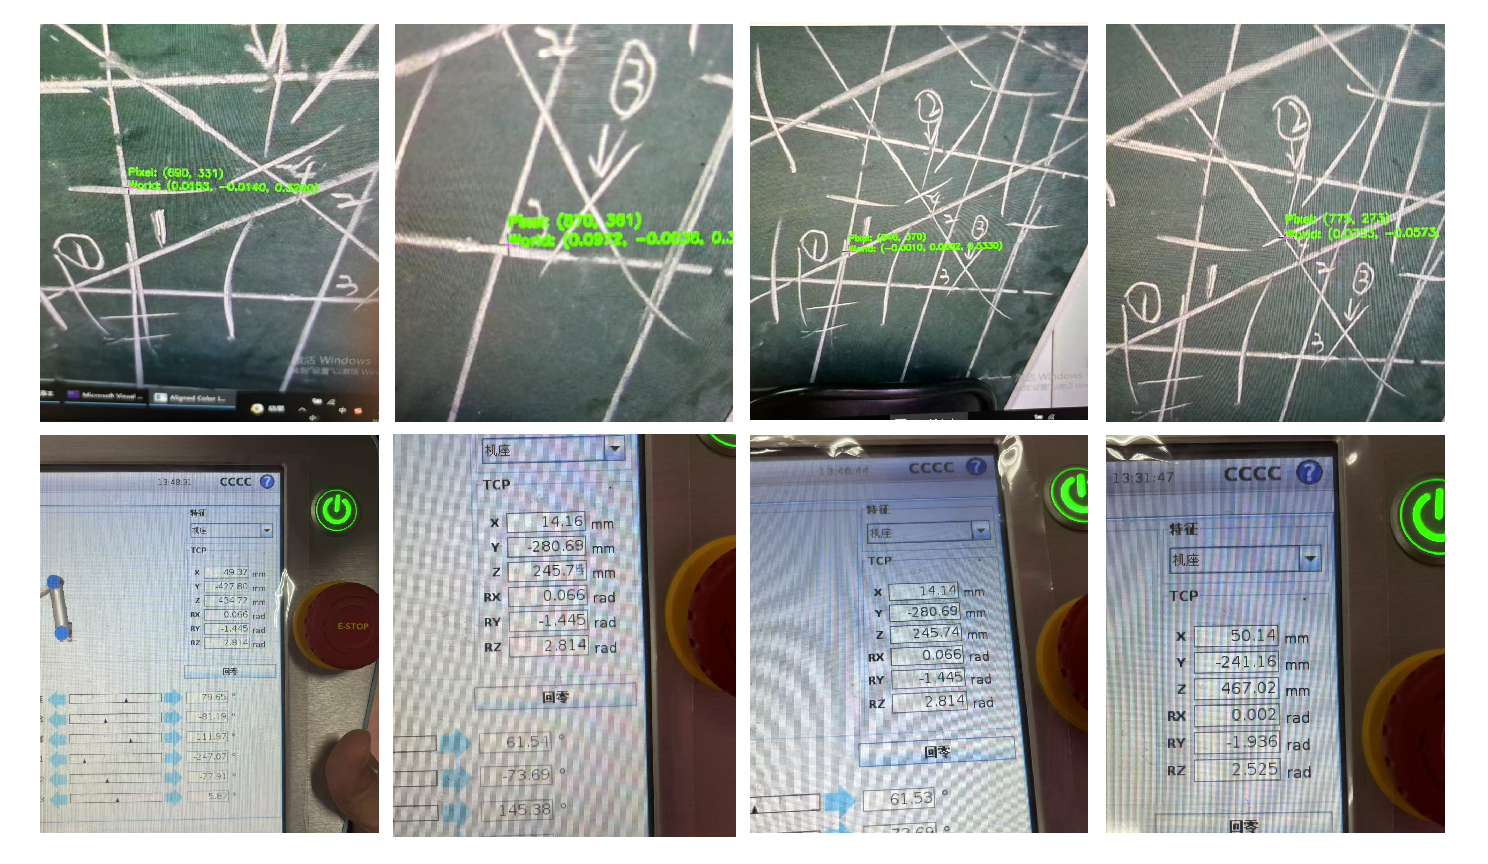
\includegraphics[width=0.8 \textwidth]{eye-in-hand.drawio.png}
	\caption[采集标定数据示例图]{采集标定数据示例图} % 中括号中内容为插图索引中显示内容,可在题注内容过长时使用
	\label{eye-in-hand1}
\end{figure}

在实验中,手眼标定用于确定相机坐标系与机械臂末端坐标系之间的变换关系,以确保机械臂能够基于视觉感知信息进行精确操作。本实验采用 Eye-in-Hand(眼在手上) 配置,即在机械臂(UR5)的末端安装 Intel RealSense D435i 深度相机,使相机与机械臂同步运动,从不同角度观察目标物体。为保证标定的精度,实验通过多次数据采集,计算出相机相对于机械臂末端的位姿变换矩阵。

数据采集的核心步骤包括机械臂运动控制、图像采集、位姿记录和数据存储。首先,机械臂按照预设轨迹移动至不同位置,每个位置的相机视角不同,以确保标定数据的多样性。在每个位姿点,深度相机拍摄目标点位图像,并使用 OpenCV 进行角点检测,从而获取目标点位在相机坐标系下的三维坐标信息。同时,机械臂的关节编码器记录当前末端在基座坐标系下的位置与姿态,形成完整的数据对,如\cref{eye-in-hand1}所示。所有采集的数据存储为结构化格式,包括机械臂末端的位姿矩阵和相机观测到的目标点位坐标向量,以便后续计算。

在数据采集过程中,为了保证标定精度,实验采取了一系列质量控制措施。首先,确保目标点位在不同视角下均能被完整检测,避免数据偏差。其次,控制机械臂的运动稳定性,避免因震动或误差积累影响标定结果。对于图像采集环节,实验检查角点检测的稳定性,若发现某些视角的检测误差较大,则重新采集数据,以确保输入数据的准确性。

\subsubsection{深度图像数据采集}
本章实验中深度图像数据来自\ref{sec:dataset}中的数据集,故在此不重复叙述。

\subsection{实验设计}
本实验旨在提高机器人视觉系统的感知能力,通过深度图像噪声处理、手眼标定及目标朝向估计优化位姿计算精度,为机器人精准操作提供可靠的数据支持。实验主要涵盖三个部分,分别针对深度数据质量优化、相机与机械臂坐标转换精度评估以及目标朝向预测准确性进行验证。

在深度图像噪声处理实验中,首先采集多个场景的深度图像,包括光滑表面、复杂纹理表面以及具有透明、反射特性的物体,以分析不同目标的深度噪声特性。实验在稳定光照和变化光照环境下进行,评估深度图像的误差分布、空洞区域及边界失真情况。为了提升深度数据质量,实验采用 密度峰值去噪方法,对比 双边滤波 和 中值滤波 的去噪效果,统计去噪前后点云的完整性、曲面平滑度以及误差降低幅度。预期结果是密度峰值去噪能显著减少噪声点,提高点云的连续性,从而优化机器人基于深度信息的三维重建效果。

在手眼标定实验中,实验采用 Eye-in-Hand(眼在手上) 配置,即在机械臂末端安装深度相机,随机械臂运动观察标定板,以求解相机坐标系到机械臂末端坐标系的变换矩阵。实验选取 10-20 个不同位姿 采集数据,记录机械臂末端的运动轨迹,并通过 OpenCV 计算目标点位在相机坐标系下的位姿信息。随后,实验采用最小二乘优化算法 计算变换矩阵,并评估其误差,主要包括平移误差和旋转误差。

在目标朝向估计实验中,实验采集不同朝向的番茄花 RGB-D 图像,并手动标注其真实朝向(上、下、左、右、前)。采用 YOLACT 目标检测网络 进行目标分割,并结合 环形平滑标签(CSL)方法 预测朝向,以减少传统数值回归方法的边界误差问题。实验设计对比 CSL 方法和数值回归方法的分类准确率,并分析误分类情况,统计误分类角度的分布范围。


\subsection{实验结果与分析}
\subsubsection{深度图像去噪}
\begin{table}[htbp]
	\centering
	\caption[连续像素区域去噪前后数值对比]{连续像素区域去噪前后数值对比}
	\begin{tabularx}{\textwidth}{YYY}
		\toprule
		\textbf{序号} & \textbf{去噪前(深度 mm)} & \textbf{去噪后(深度 mm)} \\
		\midrule
		1  & 354.21 & 354.21 \\
		2  & 354.20 & 354.20 \\
		3  & 354.19 & 354.19 \\
		4  & 354.20 & 354.20 \\
		5  & 354.20 & 354.20 \\
		7  & \textcolor{red}{675.89} & 354.20 \\
		8  & \textcolor{red}{675.90} & 354.20 \\
		9  & 354.18 & 354.18 \\
		10 & 354.19 & 354.19 \\
		11 & 354.21 & 354.21 \\
		\bottomrule
	\end{tabularx}
	\label{tab:noise1}
\end{table}

深度图像去噪的主要目的是去除噪声异常点,减少因环境影响导致的深度数据突变,使深度图像更加平滑。\cref{tab:noise1}表示使用密度峰值去噪后,一组连续像素点去燥前后的数值变化。

实验结果表明,在去噪前,该区域的大部分深度值稳定在 354.20 mm 左右,但在第 7 和 8 行 出现了异常深度值 675.89 mm 和 675.90 mm,远超周围像素点的数值范围。这些异常点可能是由于空洞、环境光照干扰或物体材质特性导致的。经过密度峰值去噪处理后,这些异常点被成功修正回 354.20 mm,与周围像素值保持一致,而原本正常的深度数据未受影响。这一结果说明,密度峰值去噪方法能够精准检测并修正异常值,同时保持正常数据的完整性,避免对整体深度图像造成额外干扰。
\begin{table}[htbp]
	\centering
	\caption[局部区域去噪前后均方误差和方差]{局部区域去噪前后均方误差和方差}
	\begin{tabularx}{\textwidth}{YYY}
		\toprule
		\textbf{去噪阶段} & \textbf{均方误差(MSE)} & \textbf{方差(Variance)} \\
		\midrule
		去噪前 & 2.21 & 1.18 \\
		去噪后 & 1.66 & 0.79 \\
		\bottomrule
	\end{tabularx}
	\label{tab:noise2}
\end{table}


为了进一步量化去噪方法的效果,实验计算了去噪前后的均方误差和 方差,如\cref{tab:noise2}所示,分别用于衡量去噪后数据与真实值的偏差,以及去噪前后深度数据的波动程度。实验结果表明,去噪前局部区域的均方误差为 2.21 mm²,去噪后降低至 1.66 mm²,误差减少 24.9\%。这表明去噪方法能够有效减少深度数据的测量误差,使其更接近真实值。此外,去噪前的方差为 1.18,去噪后降至 0.79,减少 33.1\%,表明去噪后的深度数据更加稳定,局部区域的深度波动性明显降低。

\subsubsection{空间映射}
\begin{table}[htbp]
	\centering
	\caption[用于计算手眼变换矩阵的观测数据]{用于计算手眼变换矩阵的观测数据}
	\begin{tabularx}{\textwidth}{
			>{\hsize=0.3\hsize\centering\arraybackslash}Y
			>{\hsize=1.8\hsize\arraybackslash}Y
			>{\hsize=1.1\hsize\arraybackslash}Y
			>{\hsize=0.8\hsize\arraybackslash}Y}
		\toprule
		\textbf{序号} & \textbf{TCP 坐标} & \textbf{相机坐标} & \textbf{基座标} \\
		\midrule
		1 & [14, -280, 245, 0.066, -1.445, 2.814] & [-0.002, -0.046, 0.343] & [49, -427, 434] \\
		2 & [14, -280, 245, 0.066, -1.445, 2.814] & [0.076, -0.105, 0.351]  & [-25, -419, 496] \\
		3 & [14, -280, 245, 0.066, -1.445, 2.814] & [0.097, -0.003, 0.398]  & [-50, -490, 411] \\
		4 & [14, -280, 245, 0.066, -1.445, 2.814] & [-0.001, 0.000, 0.533]  & [48, -613, 438] \\
		\bottomrule
	\end{tabularx}
	\label{tab:eye-in-hand2}
\end{table}


为了提高标定精度,本实验首先对采集数据进行筛选,剔除误差较大的数据点。采用3σ 原则对数据误差进行筛选,即剔除误差超过均值 ±3 倍标准差的点,并利用欧氏距离检测剔除突变点, \cref{tab:eye-in-hand2}为剔除突变后的一组数据。数据筛选完成后,使用\cref{equ:hand-in-eye2}计算相机坐标系到机械臂末端坐标系的变换矩阵$X$,随后采用重投影误差评估标定精度,验证优化后的标定矩阵转换的精度,由\cref{equ:hand-in-eye3}计算重投影后目标点的坐标。
\begin{equation}
	\label{equ:hand-in-eye3}
	T = T_{tcp}^{base} \cdot T_{target}^{camera} \cdot X
\end{equation}

其中 $T_{tcp}^{base}$为tcp坐标,$T_{target}^{camera}$为目标点位的相机坐标,$X$为计算的到手眼转换矩阵。
\begin{table}[htbp]
	\centering
	\caption[重投影坐标与真实坐标对比]{重投影坐标与真实坐标对比}
	\begin{tabularx}{\textwidth}{YYY}
		\toprule
		\textbf{观测点位} & \textbf{重投影坐标(m)} & \textbf{真实坐标(m)} \\
		\midrule
		1 & [0.0404, -0.0453, 0.4220] & [0.0402, -0.0450, 0.4219] \\
		2 & [0.0972, -0.0038, 0.3980] & [0.0971, -0.0037, 0.3983] \\
		3 & [0.0752, -0.0573, 0.5390] & [0.0753, -0.0572, 0.5390] \\
		4 & [-0.2000, 0.0226, 0.3872] & [-0.2002, 0.0224, 0.3873] \\
		\bottomrule
	\end{tabularx}
	\label{tab:eye-in-hand3}
\end{table}
 \cref{tab:eye-in-hand3}为一组重投影坐标与真实坐标对比。实验结果表明,重投影坐标与真实坐标的误差极小,例如,第一个观测点的重投影坐标为 $[0.0404, -0.0453, 0.4220]$,而真实坐标为 $[0.0402, -0.0450, 0.4219]$,误差控制在 0.3 mm 以内。所有观测点的最大误差均不超过 0.5 mm,表明标定矩阵计算精确,适用于高精度任务。实验结果进一步证明,优化后的标定矩阵能够有效减少误差,使机械臂在不同视角下能够精准感知目标物体的位置。
 
 \section{本章小节}
 本章提出了一种基于对称虚拟空间的位姿重建方法,旨在解决农业场景中机械臂授粉任务对三维感知精度与实时性的双重需求。通过引入密度峰值去噪方法,显著提升了深度图像的稳定性与重建精度,有效剔除异常点并增强点云一致性。在手眼标定过程中,构建了Eye-in-Hand系统架构,采用多位姿数据采集与误差优化策略,实现了高精度的坐标系变换矩阵求解。针对番茄花多样朝向的挑战,采用环形平滑标签方法,将姿态估计转化为分类问题,结合YOLACT目标检测模型高效预测目标朝向。
 
 实验在不同光照和背景条件下验证了所提方法的鲁棒性与实用性,深度去噪使得局部区域均方误差减少24.9\%,方差降低33.1\%;手眼标定误差控制在0.5mm以内;目标朝向分类方法展现出更高的稳定性和抗干扰能力。整体系统能够为后续的授粉路径规划与柔顺控制提供高质量的三维位姿数据支撑。